% Auto-generated by figures/make_figures.py.

\begin{figure*}[t]
  \centering
  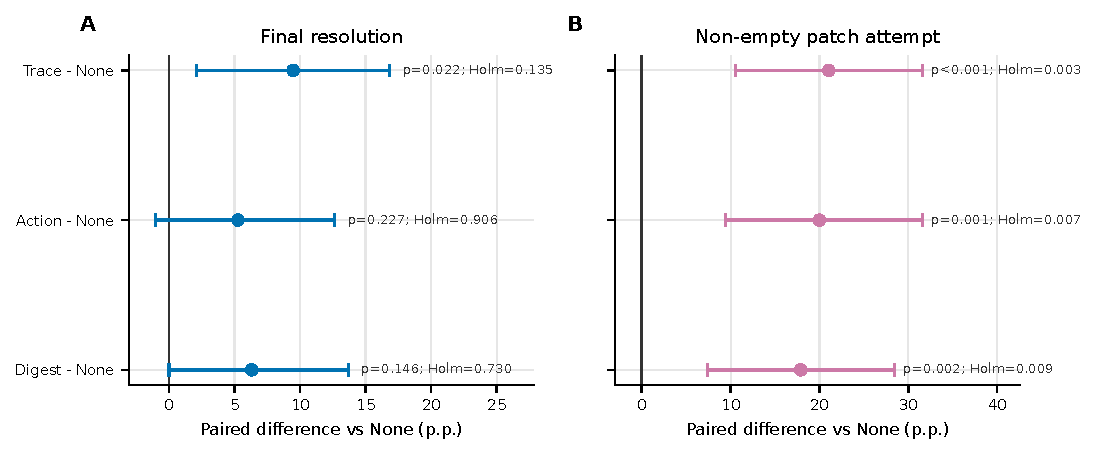
\includegraphics[width=\linewidth]{figures/fig_paired_effects.pdf}
  \caption{\textbf{Paired effects versus no prior context.} Points show paired percentage-point differences against None with paired bootstrap 95\% intervals. Resolution gains are descriptive and paired-success McNemar tests are not Holm-significant, while non-empty patch-attempt effects are large and Holm-significant. These comparisons do not imply causal mediation.}
  \label{fig:paired-effects}
\end{figure*}

\begin{figure*}[t]
  \centering
  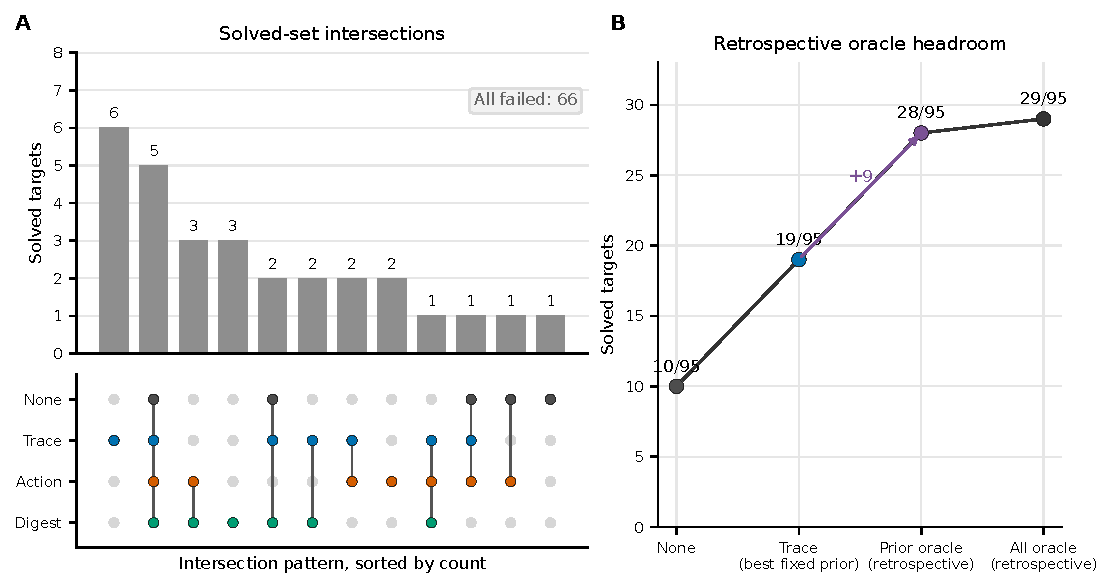
\includegraphics[width=\linewidth]{figures/fig_solve_complementarity_oracle.pdf}
  \caption{\textbf{Solve complementarity and retrospective oracle headroom.} Trace has the highest fixed prior-context solve count, but different prior representations solve different targets. A retrospective prior-context oracle reaches 28/95, which is +9 over the best fixed prior representation, while the all-condition retrospective oracle reaches 29/95. The oracle is retrospective and not a deployable method.}
  \label{fig:solve-complementarity-oracle}
\end{figure*}

\begin{figure*}[t]
  \centering
  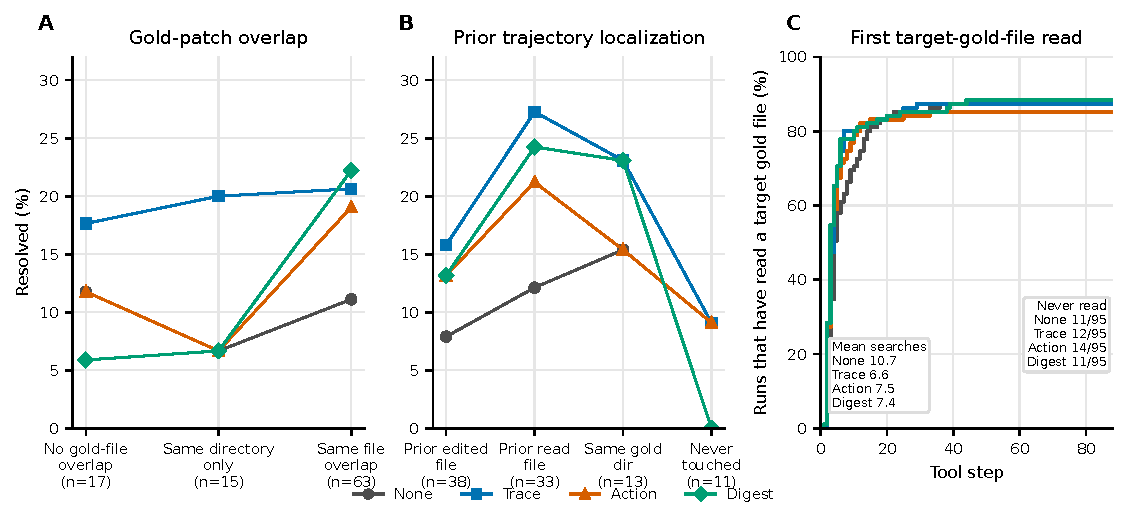
\includegraphics[width=\linewidth]{figures/fig_localization_map.pdf}
  \caption{\textbf{Localization map.} Prior-context gains concentrate when prior and target trajectories are local in file or directory space. The ECDF denominator is all 95 targets per condition; runs with missing first target-gold-file reads are counted as never reached. Prior-context agents reach target-gold files earlier and use fewer mean search commands, consistent with localization/procedural transfer rather than proving a causal mechanism.}
  \label{fig:localization-map}
\end{figure*}

\begin{figure*}[t]
  \centering
  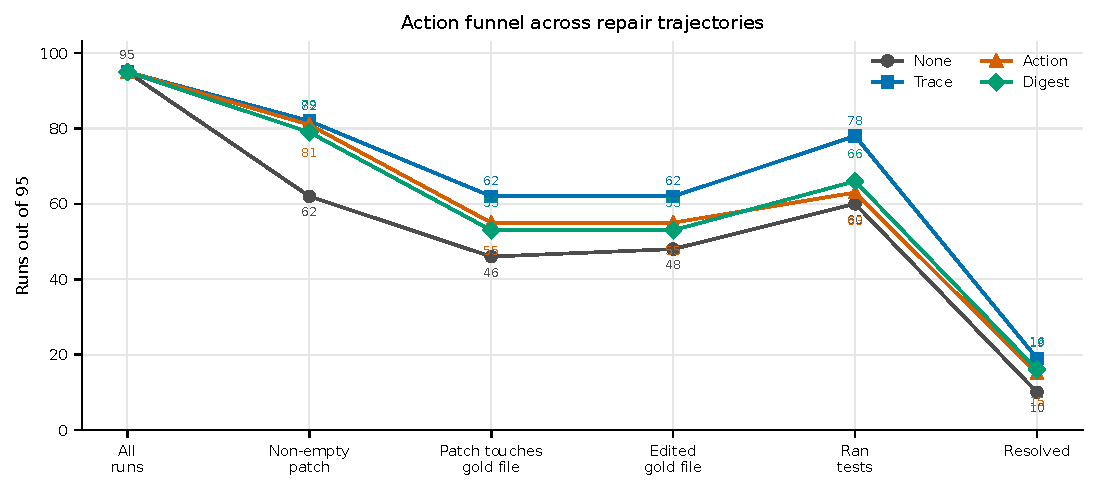
\includegraphics[width=\linewidth]{figures/fig_patch_action_funnel.pdf}
  \caption{\textbf{Patch/action funnel.} Prior-context conditions primarily reduce empty-patch behavior and increase target-relevant actions before the narrower final-resolution endpoint. Because running tests is not strictly sequential after editing, this is an action funnel rather than a causal pipeline.}
  \label{fig:patch-action-funnel}
\end{figure*}

\begin{figure*}[t]
  \centering
  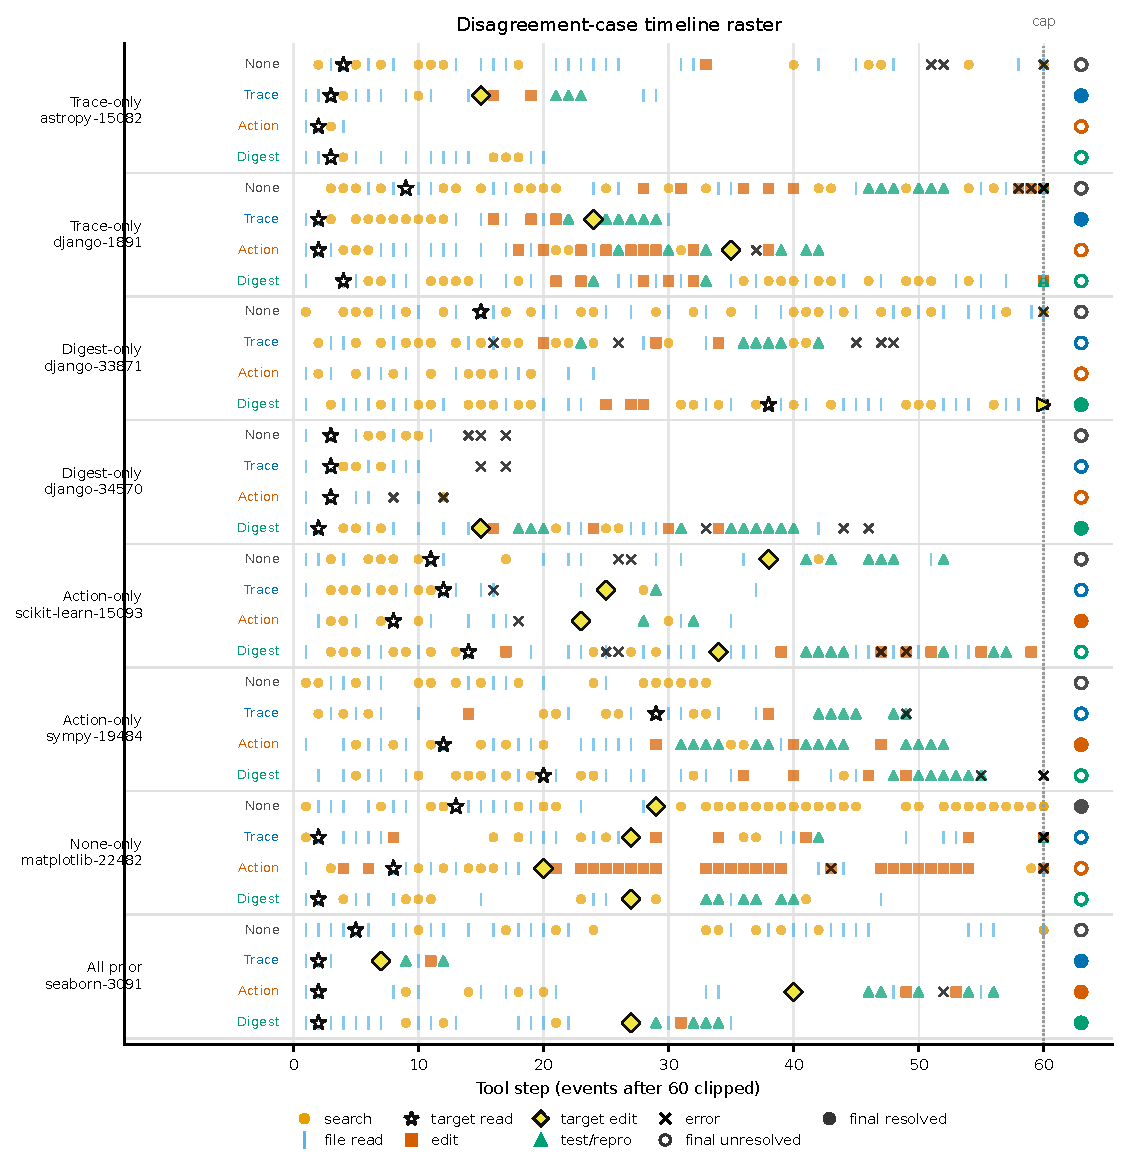
\includegraphics[width=\linewidth]{figures/fig_disagreement_timeline_raster.pdf}
  \caption{\textbf{Disagreement-case timeline raster.} Selected targets where representations disagree show that different memory renderings can route the agent through different evidence and action paths on the same target. Tool steps are capped at 60 for compactness, and snippets are omitted from the main figure.}
  \label{fig:disagreement-timeline-raster}
\end{figure*}

\begin{figure*}[t]
  \centering
  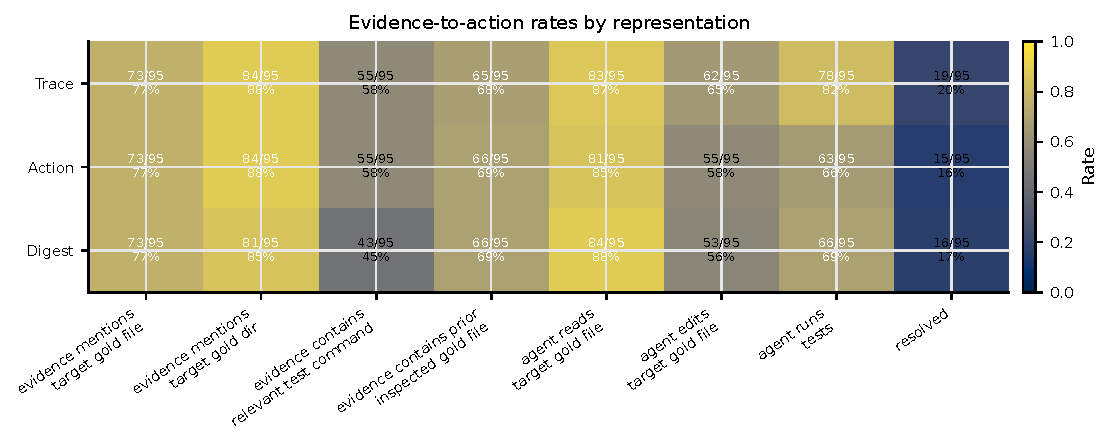
\includegraphics[width=\linewidth]{figures/appendix_fig_evidence_action_heatmap.pdf}
  \caption{\textbf{Evidence-to-action heatmap.} Representation-exposed evidence is often present, but evidence presence is not sufficient for success; the agent must read, edit, test, and ultimately resolve. This post hoc analysis is descriptive and not causal.}
  \label{fig:evidence-action-heatmap}
\end{figure*}
